\documentclass[11pt,a4paper]{article}

% --- Packages ---
\usepackage[utf8]{inputenc}
\usepackage[T1]{fontenc}
\usepackage{geometry}
\geometry{margin=1in}
\usepackage{xcolor}
\usepackage{listings}
\usepackage{tikz}
\usetikzlibrary{shapes.geometric, arrows, positioning, shadows}
\usepackage{hyperref}
\usepackage{booktabs}

% --- Font Fallback ---
\renewcommand{\familydefault}{\sfdefault} % Use standard sans-serif

% --- Custom Colors ---
\definecolor{lushioblue}{HTML}{0056b3}
\definecolor{pwcgrey}{HTML}{4d4d4d}
\definecolor{codebackground}{HTML}{f8f9fa}

% --- Custom Commands ---
\newcommand{\mysection}[1]{%
    \vspace{0.4cm}%
    {\color{lushioblue}\Large\bfseries #1}%
    \par\vspace{0.2cm}%
}
\newcommand{\mysubsection}[1]{%
    \vspace{0.3cm}%
    {\color{pwcgrey}\large\bfseries #1}%
    \par\vspace{0.1cm}%
}

% --- Code Styling ---
\lstset{
    backgroundcolor=\color{codebackground},
    basicstyle=\ttfamily\small,
    breaklines=true,
    commentstyle=\color{gray},
    keywordstyle=\color{lushioblue},
    stringstyle=\color{orange},
    frame=single,
    rulecolor=\color{lightgray},
    xleftmargin=10pt,
}

% --- TikZ Styles ---
\tikzstyle{startstop} = [circle, minimum width=1.5cm, minimum height=1cm, text centered, draw=black, fill=red!30, drop shadow]
\tikzstyle{process} = [rectangle, minimum width=3cm, minimum height=1cm, text centered, rounded corners, draw=black, fill=blue!10, drop shadow]
\tikzstyle{decision} = [diamond, minimum width=3cm, minimum height=1cm, text centered, draw=black, fill=green!10, drop shadow]
\tikzstyle{arrow} = [thick,->,>=stealth]
\tikzstyle{database} = [cylinder, cylinder uses custom fill, cylinder body fill=gray!10, cylinder end fill=gray!20, shape border rotate=90, draw, minimum height=1.5cm, minimum width=1.2cm, drop shadow]

\begin{document}

% --- Title ---
\begin{center}
    {\Huge \textbf{Lushio AI: Deep Technical Architecture}} \par
    \vspace{0.5cm}
    {\large \textit{A Comprehensive Deep-Dive into Multi-Agent Orchestration \& RAG}} \par
    \vspace{1cm}
\end{center}

\mysection{Executive Summary}
Lushio AI represents a shift from linear procedural pipelines to autonomous agentic workflows. Built on \textbf{LangGraph}, the system leverages a supervisor-led multi-agent architecture to handle complex retail inventory and policy queries. This document details the underlying state machine, retrieval strategies, and the technical safeguards ensuring high-fidelity outputs.

\mysection{1. Orchestration: The DAG with Feedback Loops}
Unlike traditional "chain-of-thought" systems, Lushio employs a graph-based orchestration model. This allows for conditional branching and iterative loops, which are critical for accuracy when initial research is insufficient.

\mysubsection{The Role of the Supervisor}
The Supervisor node acts as the "brain," performing an initial intent-classification on the user query. It dynamically generates a directive for the Research agent. By isolating intent-parsing from tool-execution, the system reduces the risk of tool-misuse by smaller, more specialized agents.

\mysubsection{Evaluation \& Iteration Control}
A critical technical component is the \texttt{evaluate\_research} node. It functions as a semantic gatekeeper. 
\begin{itemize}
    \item \textbf{Semantic Completeness}: It compares the gathered evidence against the original user requirements. If gaps are found, it routes back to the Researcher.
    \item \textbf{Loop Prevention}: It enforces a strict iteration limit to ensure the graph reaches a terminal state (The Writer) and prevents costly "infinite reasoning loops."
\end{itemize}

\begin{center}
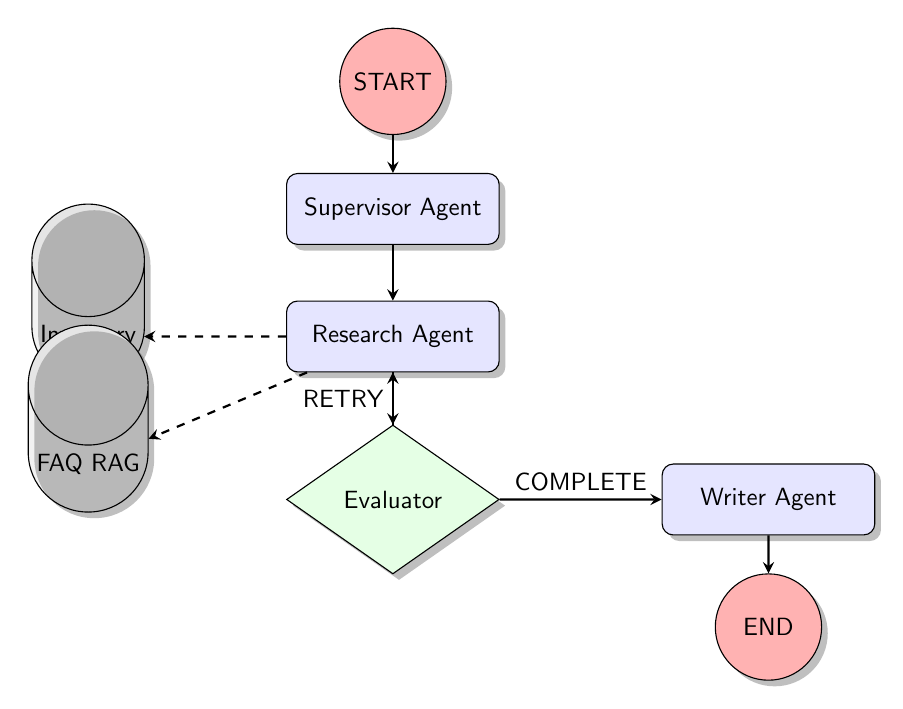
\begin{tikzpicture}[node distance=1.8cm, scale=0.9, every node/.style={scale=0.9}]
    \node (start) [startstop] {START};
    \node (sup) [process, below of=start] {Supervisor Agent};
    \node (res) [process, below of=sup] {Research Agent};
    \node (eval) [decision, below of=res, yshift=-0.5cm] {Evaluator};
    \node (writer) [process, right of=eval, xshift=3.5cm] {Writer Agent};
    \node (end) [startstop, below of=writer] {END};
    
    \node (db) [database, left of=res, xshift=-2.5cm] {Inventory};
    \node (rag) [database, below of=db] {FAQ RAG};

    \draw [arrow] (start) -- (sup);
    \draw [arrow] (sup) -- (res);
    \draw [arrow] (res) -- (eval);
    \draw [arrow] (eval) -- node[anchor=east] {RETRY} (res);
    \draw [arrow] (eval) -- node[anchor=south] {COMPLETE} (writer);
    \draw [arrow] (writer) -- (end);
    
    \draw [arrow, dashed] (res) -- (db);
    \draw [arrow, dashed] (res) -- (rag);
\end{tikzpicture}
\end{center}

\mysection{2. State Management: The Immutable Blackboard}
Lushio follows the "Blackboard" architectural pattern. The \texttt{AgentState} is a persistent shared object that evolves as it moves through the graph.

\mysubsection{Strict Typing for Traceability}
The use of \texttt{TypedDict} ensures that every node has a clear contract. This is vital for debugging in production; developers can inspect the state at any node to understand \textit{why} a specific decision was made.

\begin{lstlisting}[language=Python]
class AgentState(TypedDict):
    query: str                  # Original user input
    supervisor_directive: str   # Intent deconstruction
    inventory_items: List[Dict] # Extracted structured data
    research_data: str          # Unstructured RAG results
    research_iterations: int    # Guard for max loops
    final_answer: Dict[str,Any] # The validated hand-off
\end{lstlisting}

\mysection{3. Advanced Retrieval (RAG) \& Tool-Access}
The system bridges the gap between structured JSON databases (for inventory) and unstructured vector search (for policies).

\begin{itemize}
    \item \textbf{Hybrid Discovery}: The Research agent uses fuzzy matching via tools to query the local JSON store, allowing for flexible product lookups.
    \item \textbf{Vectorized Knowledge}: Utilizing \texttt{all-MiniLM-L6-v2} embeddings, the system maintains a semantic index in Pinecone, enabling rapid policy lookups for returns and shipping.
\end{itemize}

\mysection{4. Technical Resilience \& Production Roadmap}
The architecture is designed for the \textbf{PwC GenAI Standard}, prioritizing ROI through reliability.

\mysubsection{Planned Hardening (Production Roadmap)}
The following features are currently being prioritized to meet full enterprise production requirements:
\begin{enumerate}
    \item \textbf{Token Truncation}: Monitoring research data size to prevent context window overflow.
    \item \textbf{Async Invocation}: Migrating from \texttt{invoke} to \texttt{ainvoke} to support high-concurrency workloads.
    \item \textbf{Tool Retries}: Implementing exponential backoff for tool connections to handle transient network issues.
\end{enumerate}

\vspace{1cm}
\begin{center}
\fbox{
\begin{minipage}{0.9\textwidth}
\textbf{Conclusion} \par
Lushio AI's architecture provides a scalable foundation for retail intelligence. By combining strict state management with autonomous orchestration, the system delivers high accuracy while maintaining the traceability required for enterprise compliance.
\end{minipage}
}
\end{center}

\end{document}
